\label{subsec:case_studies}

\begin{table*}
\centering
\begin{tabular}{l|l|l|l|l|}
Bug Name & Topology & Replay Success Rate & MCS Size & Final MCS replayable? \\
\hline
Newly found Bugs & - & - & - & - \\
\hline
Pyretic loop & 3 switch mesh & 20/20 & 2 & Yes \\
% experiments/new_pyretic_loop_mcs/
% Total original inputs: 36
POX in-flight blackhole & 2 switch mesh & 15/20 [20/20*] & 11 & Yes \\
% Total inputs: 26
% With DP events: 68/25
% Original: 7ba95ed82ca4e32f12ab511d9c4301dbac2c59d5
% MCS: 399cf861db87a65e600283d9ae7760400c4676e2
% Updated: updated_debug_branch_loop/
% TODO(cs): move to "known bugs"?
POX premature handshake & 4 switch mesh & 20/20 & 2 & Yes \\
% Andi: experiments/pox_early_packetin
% Total inputs: 102
POX migration blackhole & 4 switch mesh & 20/20 & 3 & Yes \\
% Total inputs: 29
% With DP events: 117/3
% fuzz_pox_4mesh_blackhole
% Updated (fat tree): pox_fattree_migration
POX list removal & 2 switch mesh & 20/20 & 2 & Yes \\
% Total inpujts: 69
% With DP events: 72/2
% Original: config/eugene_epsilon_replay.py
% MCS: config/eugene_epsilon_mcs.py
NOX discovery loop & 4 switch mesh & 18/20 & 18 & No \\
% Total inputs: 150
% With DP events: 358/58
% Original: ce547fc1df3bde279b6f3dd589c909663e295f1e
% MCS: 5f49e791b0c1a611454cf0930f54aa609dd635d3
% Updated to new format: nox_mesh_4_loop_repro_verbose
Floodlight loop & 3 switch mesh & 15/50 & 36 & Yes \\
% Total inputs: 284
% Andi
ONOS distributed database locking & 2 switch mesh & TBD & 3 & Yes \\
% Ahmed
\hline
Known Bugs & - & - & - & - \\
\hline
Floodlight example failover bug & 2 switch mesh & - & 2 & Yes \\
% Predates the experiment directory
ONOS master election & TBD & - & TBD & TBD \\
% Ahmed
Load Balancer Flow Table Space & 3 switch mesh & - & 24 (N+1) & Yes \\
% load_balancer_fuzzer_mcs/
% Total original inputs: 106
% --------
%ONOS forgotten flows & TBD & TBD & TBD \\
\hline
Synthetic Bugs & - & - & - & - \\
\hline
Null pointer on rarely used codepath & 20 switch FatTree & - & 2 & Yes \\
% experiments/experiments/pox_null_pointer_mcs
% total original inputs: 365
Overlapping flow entries & 2 switch mesh & - & 2 & Yes \\
% experiments/trigger_priority_mismatch_small_mcs
% total original inputs: 27
Delicate timer interleaving & 3 switch mesh & - & 39 & No \\
% experiments/snapshot_demo_synthetic_link_failure
% total original inputs: 39
Algorithm misimplementation & 3 switch mesh & - & 7 & No \\
% experiments/experiments/pox_broken_floyd_mcs
% total original inputs: 40
% MCS is inflated! link failure / recovery in MCS not related to triggering events.
Multithreaded race condition & 10 switch mesh & - & 2\footnote{The race
condition triggered by any I/O events, so the final MCS was essentially
random} & Yes\footnote{With multiple replays per subsequence} \\
% experiments/trigger_multithreading_bug_mcs
% total original inputs: 1596
Memory Leak & 2 switch mesh & - & 30 (M) & No \\
% experiments/trigger_memory_leak3_mcs/
% total original inputs: 719
%Execution-speed race condition & 3 switch mesh & - & 9 & Yes \\
%% "floodlight" branch: experiments/floodlight_loop_2014_mcs_*
%% Total original inputs: 157
Memory Corruption & 4 switch mesh & - & 2 & Yes \\
% syn_mem_corruption_3switch_fuzzer_mcs
% Total original inputs: 341
% ----
%Ignored Bad OpenFlow args & TBD & TBD & TBD \\
%Latency spike & TBD & TBD & TBD \\
%Invalid sleep value & TBD & TBD & TBD \\
%Non-deterministic TCAMs -> transient tenant isolation breach & TBD & TBD & TBD \\
%Decision based on last byte of TCP SYN & TBD & TBD & TBD \\
\end{tabular}
\caption{Overview of Case Studies. \newline
\textmd{*with multiplexed sockets, overridden {\tt gettimeofday()}, and
logging interposition enabled.}}
\label{tab:case_studies}
\end{table*}

Our goal in this section is to show that \projectname~successfully produces
MCSes that are useful for troubleshooting. The
gold standard for evaluating \projectname~would be a large scale A/B test~\cite{neyman}
showing how much time it takes for developers to troubleshoot bugs found in
QA clusters with and without minimized event traces. Unfortunately
expert developers are scarce, and their skills vary widely; to achieve statistical significance we would
need hundreds of developers to spend substantial time on each bug we find.
%We also lack access to bugs found by QA testbeds of the scale and complexity
%used to test production controller software.

We instead take two approaches to evaluating \projectname.
First, we demonstrate \projectname's viability in
troubleshooting real bugs. We found \num{eight} new bugs by fuzz testing open source
SDN control platforms:
ONOS~\cite{ONOS} (Java), POX~\cite{pox} (Python), NOX~\cite{nox} (C++),
Pyretic~\cite{frenetic} (Python), and Floodlight~\cite{bigswitch} (Java), and
debugged these with the help of \projectname. Second, we demonstrate the
boundaries of where \projectname~works well and where it does not by finding
MCSes for previously known and synthetic bugs that span a range of bug types encountered in
practice. Throughout our evaluation
we quantitatively show \projectname's ability to minimize traces, and we
qualitatively demonstrate the use of MCSes for troubleshooting.

We show a high-level overview
of our results in Table~\ref{tab:case_studies}, and
illustrate in detail how \projectname~found their minimal causal sequences
in the rest of this section. Interactive visualizations and replayable event traces
for all of these case studies are publicly available (anonymized).

\subsection{New Bugs}
% \href{http://ucb-sts.github.com/experiments}{ucb-sts.github.com/experiments}.

\noindent{\bf POX List Removal.} The first
SDN controller we examined was POX. %the successor of NOX. POX is
%a single-machine control platform intended primarily for research prototyping
%and educational use (\ie~not large scale production use). Nevertheless, POX has
%been deployed on real networks, and has a growing set of users.
The POX application we ran was a layer two routing module (`l2\_multi') that
learns host locations and installs exact match per-flow paths between known
hosts, after discovering links in the network. %, and a spanning tree module,
%which configures switches to only flood packets for unknown hosts along a
%spanning tree.

We start with a simple bug. %to illustrate that
%\projectname~is useful for early stage development and testing.
We generated random sequences of
inputs, and found after some time that POX threw an exception due to
attempting to remove an element from a list where the element was not present.

There were $69$ randomly generated inputs in the trace leading up to the
exception. We invoked \projectname~to identify a two element MCS (runtime
shown in Figure~\ref{fig:list_runtime}):
a failure of a connected switch followed by a reboot/initialization of the same switch.
The stack trace made it easy to identify the code path that
immediately preceded the exception, and with
the knowledge that the initial triggering event was a switch failure we were able to
find why the original element was inserted into the list and fix the
problem within 15 minutes.

\begin{figure}[t]
    %\hspace{-10pt}
    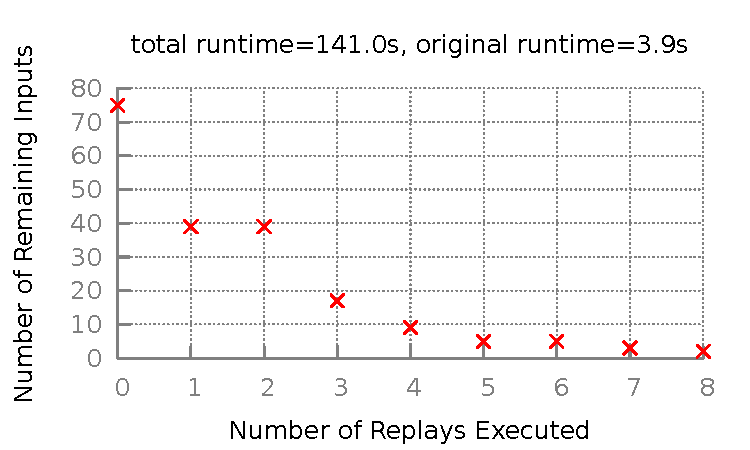
\includegraphics[width=3.25in]{../graphs/runtime/list_remove_error.pdf}
    \caption[]{\label{fig:list_runtime} Minimizing the POX list remove trace.}
\end{figure}

\eat{ % -----------------------------------
Apparently the developers of POX had not anticipated this particular event
sequence. Given the rarity of switch recovery events, and the tediousness of
writing unit tests for scenarios such as this
(which involved multiple OpenFlow initialization handshakes), this is not
surprising.
%Consider that the state-of-the-art open source technology for prototyping SDN
%applications, Mininet~\cite{handigol2012reproducible}, excels at
%testing common scenarios (on production OpenFlow software switches),
%but is not explicitly designed for scripting corner-case scenarios such as
%switch failure/recovery.
\projectname~made it straightforward to inject inputs
at a high semantic level,
and the minimized event
trace it produced made for a simple integration test.
} % -----------------------------------

%We illustrate type errors to show how STS is a useful framework for exploring
%code paths that you forget to unit tests.

\noindent{\bf POX Premature Handshake.} Andi, TBD.
Runtime in Figure~\ref{fig:pox_handshake}.

\begin{figure}[t]
    %\hspace{-10pt}
    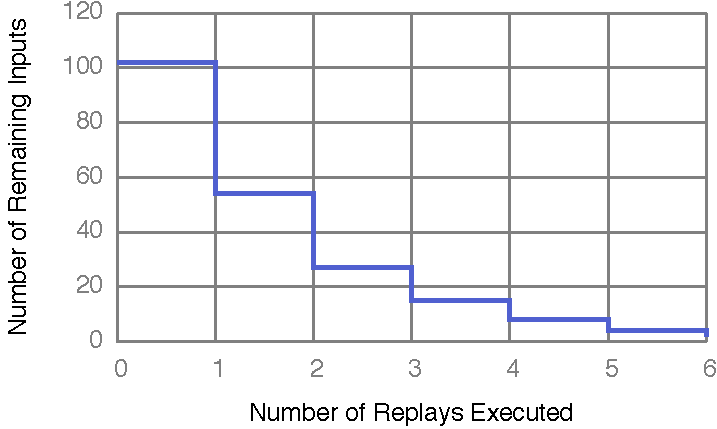
\includegraphics[width=3.25in]{../graphs/runtime/pox_early_packetin.pdf}
    \caption[]{\label{fig:pox_handshake} Minimizing the POX premature handshake.}
\end{figure}

\noindent{\bf POX In-flight Blackhole.} We
discovered the next bug after roughly 20 runs of randomly generated inputs.
We noticed a persistent blackhole while POX was bootstrapping its
discovery of link and host locations. There were $29$ inputs in the initial trace, and \projectname~returned a $11$ input
MCS (runtime shown in Figure~\ref{fig:pox_discovery}).

\begin{figure}[t]
    %\hspace{-10pt}
    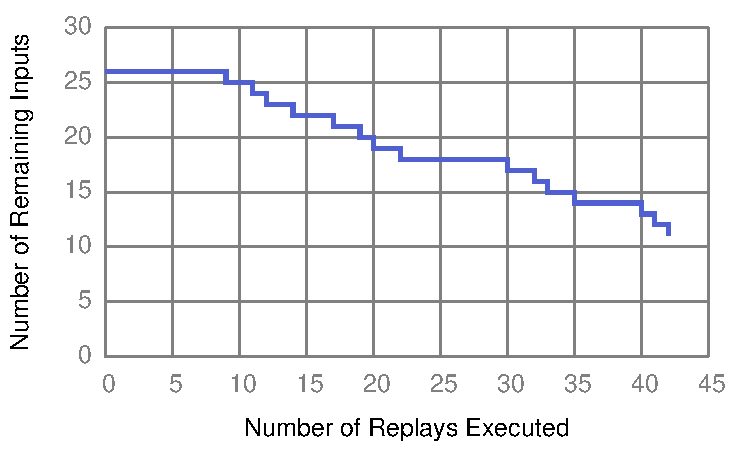
\includegraphics[width=3.25in]{../graphs/runtime/pox_blackhole.pdf}
    \caption[]{\label{fig:pox_discovery} Minimizing the POX in-flight blackhole.}
\end{figure}

We provided the MCS to the lead developer of POX. Primarily using the
console output, we were able to trace through the code and identify the problem
within 7 minutes, and were able to find a fix for the race condition within 40
minutes. By matching the console output with the code, he found that the crucial
triggering events were two
in-flight packets (set in motion by prior traffic injection events):
POX first incorrectly learned a host location as a result of the first in-flight
packet showing up immediately after POX discovered that port belonged to
a switch-switch link---apparently the code had not accounted for the
possibility of in-flight packets directly following link discovery---and
then as a result the
second in-flight packet
POX failed to return out of a nested conditional that would have
otherwise prevented the blackholed routing entries from being installed.

\eat{ % Maybe add this in -- it goes into much more depth. % -----------------------------------
We encountered this bug
on a simple topology, depicted in Figure~\ref{fig:simple_topo}, consisting of
two hosts A and B
and two switches S1 and S2 connected by a single link.

\begin{figure}[t]
    %\hspace{-10pt}
    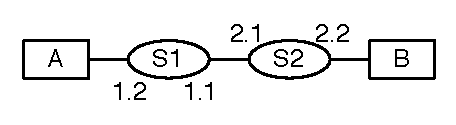
\includegraphics[width=3.25in]{../diagrams/state_machines/mesh_topo.pdf}
    \caption[]{\label{fig:simple_topo} Topology for POX
    in-flight blackhole. Numbers denote port labels.}
\end{figure}

Before the discovery module had learned of the link connecting the two
switches,
there were six traffic injection events between hosts (A$\rightarrow$ B and
B$\rightarrow$A). At the point when the link was discovered, POX had
previously learned
of B's location at port $2.2$, and correctly unlearned a previous location for
A at port $2.1$ (which it now knew to be a switch-switch link). %Upon POX would oscillate between learning the correct location
%of hosts at their ingress switch, and then learning an incorrect location
%when the flooded packet traversed the link and the next switch
%notified the controller of a new flow.\footnote{This seems to be necessary behavior before the
%links are discovered, since the hosts could have
%have legitimately migrated}
%This did not appear to be problematic though at first glance though,
%since we observed that POX correctly flushed the routing entries of the
%switches and forgot its incorrectly learned location of $A$ when it discovered
%that $1.1$ and $2.1$ were switch-switch ports, not host ports. At this point POX's only knowledge was the
%correct location of $B$ at $2.2$.

Directly after the link discovery we observed an {\em in-flight} packet arriving from A$\rightarrow$B at
port $2.1$
(without a prior flow notification from S1). This was POX's first error.
Upon examining the code, we found that it
did not account for in-flight packets concurrent with
link discovery. As a result,
POX incorrectly learned A's location at $2.1$, even though it knew that the link
could not have hosts attached. If the first packet had
instead originated at $1.1$, POX would not have made this mistake.

The next event we observed was another
{\em in-flight} packet from B$\rightarrow$A arriving at port
$1.1$. S1 notified POX of the unmatched flow, and POX appropriately printed a
log statement indicating that a packet had arrived at an internal switch port without a
previously installed flow entry. What happened next puzzled us though. POX
proceeded to install a path for this new B$\rightarrow$A flow, but the
path itself contained a loop: POX installed a B$\rightarrow$A entry going out both
$1.1\rightarrow2.1$ and $2.2\rightarrow2.1$, whereas it should have installed
only the latter (given A's current known location). The default behavior of
OpenFlow switches is to ignore matching route entries (with wildcarded in
ports) that forward out the
same port the packets arrived on. This is where we started observing the blackhole:
now whenever B sent traffic to A, it would be dropped at S1 until
the faulty routing entry would eventually expire $30$ seconds later.

We investigated the code that handled in-flight packets
arriving on switch-switch ports. The log statement that we had observed
earlier was inside a nested conditional, and the code for
installing the path was below and outside of the nested conditional.
What struck us was that there was a commented out return statement directly
after the log statement. The comment above it read: ``Should flood instead of
dropping''. We tried reinserting the return statement and replaying, and
the blackhole ceased to appear.

In summary, we found that the crucial triggering events were two
in-flight packets (set in motion by prior traffic injection events):
POX incorrectly learned a host location as a result of the first in-flight
packet, and
failed to return out of a nested conditional as a result the second in-flight
packet. We have sent the replayable trace generated by \projectname~to the lead
developer of POX, and await his response. We suspect that these fine-grained race conditions had not
been triggered before because message timing in
Mininet~\cite{handigol2012reproducible} or real hardware is not
delayed arbitrarily as it was in \projectname.

%We suspect this race condition was not observed in Mininet because the rate at which we were sending packets was
%significantly slower than in Mininet (which also sends $ARP$ and
%$IPV6$ pings), so that there were no in-flight flow notifications to POX to
%correct the situation.
% Discussion of how our gizmos helped.
} % \eat % -----------------------------------

\noindent{\bf POX Migration Blackhole.} Having
examined the POX code in some depth, we noticed that there might be
some interesting corner cases related to host migrations.
We set up randomly generated inputs, included host
migrations this time, and checked for blackholes. Our initial input size was
$29$ inputs.
\projectname produced a $3$ input MCS (shown
in Figure~\ref{fig:pox_migration}): a packet injection from a
host (`A'), followed
by a packet injection by another host (`B') towards A, followed by a host migration of A. This made it immediately
clear what the problem was. After learning the location of A and installing a
flow from B to A, the routing entries in the path were never removed after A
migrated, causing all traffic from B to A to blackhole until the routing
entries expired.
%We did not know it at the time, but this was a known problem,
%and this particular routing module did not support host migrations. Nonetheless, this
%case demonstrates how the MCS alone can point to the root cause.

\begin{figure}[t]
    %\hspace{-10pt}
    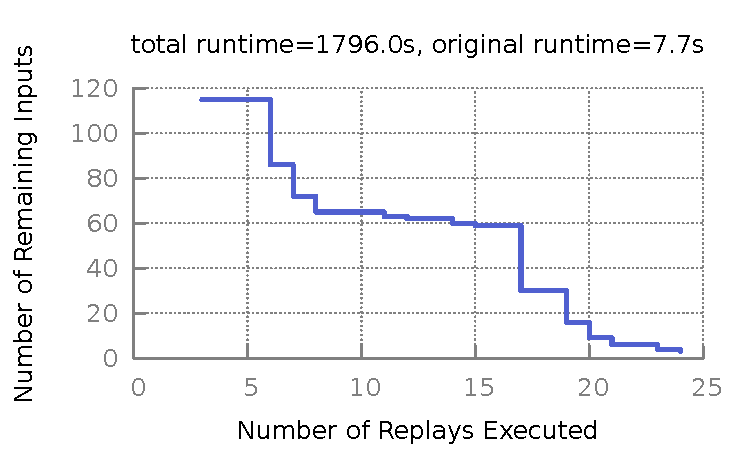
\includegraphics[width=3.25in]{../graphs/runtime/pox_migration_blackhole.pdf}
    \caption[]{\label{fig:pox_migration} Minimizing the POX migration
    blackhole.}
\end{figure}

\noindent{\bf Pyretic Loop.} We discovered a loop when fuzzing Pyretic's hub
module, whose purpose is to flood packets along a minimum spanning tree. After
minimizing the execution (runtime in figure~\ref{fig:pyretic_loop}), we found that the triggering events
were a link failure at the beginning of the trace, followed some time later by
the recovery of that link. After roughly 9 hours over two days of examining
Pyretic's (unfamiliar to us) code, we found what we believed to be the problem
in its logic for computing minimum spanning trees: it appeared that down links
weren't properly being accounted for, such that flow entries were installed
along that link even though it was down. When the link recovered, a loop was
created, as the flow entries were still in place. The loop seemed to persist until
Pyretic periodically flushed all flow entries.

\begin{figure}[t]
    %\hspace{-10pt}
    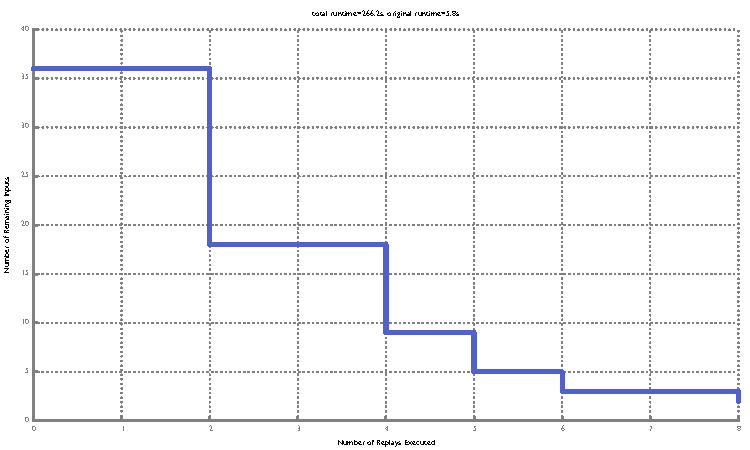
\includegraphics[width=3.25in]{../graphs/runtime/pyretic_loop.pdf}
    \caption[]{\label{fig:pyretic_loop} Minimizing the Pyretic loop.}
\end{figure}

We proceeded to file a bug report along with a replayable trace of the
minimized execution to the developers of Pyretic. They found after roughly
five hours of replaying the trace with \projectname~that Pyretic told switches to
flood out all links before the entire
network topology had been learned (including the down link). By adding a timer before installing
entries to allow for links to be discovered, the developers were able to verify
that the loop no longer appeared. A long term fix for this issue is currently being discussed by the developers of
Pyretic.

\noindent{\bf NOX Discovery Loop.} Next we tested NOX on a four-node mesh, and discovered a
routing loop between three switches within
roughly 20 runs of randomly generated inputs.

\begin{figure}[t]
    %\hspace{-10pt}
    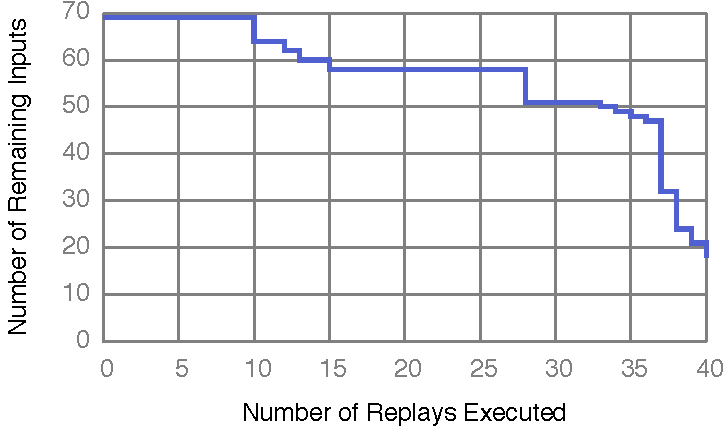
\includegraphics[width=3.25in]{../graphs/runtime/nox_loop.pdf}
    \caption[]{\label{fig:nox_discovery} Minimizing the NOX discovery loop.}
\end{figure}

Our initial input size was 68 inputs, and
\projectname~returned an 18 input MCS.
%\footnote{\num{We had difficulty
%replaying} the final MCS. The reason seems clear: this bug depends on the
%order NOX discovers links, which in turns depends on hashes computed from random memory
%addresses its discovery modules LLDP selection algorithm}
Our approach to debugging was to
reconstruct from the MCS how NOX should have installed routes, then compare
how NOX actually installed routes.

The order in which NOX discovered links was crucial: at the point NOX
installed the 3-loop, it had only discovered one link towards the destination.
Therefore all other switches routed through the one known neighbor switch.
This comprised 2 of the 3 links involved in the link.

The destination host only sent one packet, which caused NOX to initially learn
its correct location. After NOX flooded the packet though, it became confused
about its location. One flooded packet arrived at
another switch that was currently not known to be attached to anything, so NOX
incorrectly concluded that the host had migrated. Other flooded packets were
dropped as a result of link failures in the network and randomly generated
network loss. The loop was then installed when the source injected another
packet.

This case took us roughly 10 hours to debug. We are confident that without the
minimized trace, it would have taken much
longer to trace through the subtle sequence of events that were necessary for
setting up the network in precisely the right conditions.

\eat{ % -----------------------------------
The next SDN control platform we examined
was NOX, the original OpenFlow controller.
NOX is also a single machine control platform, but unlike POX it has been used
fairly extensively in real networks.

Similar to POX we exercised NOX's routing module (`sprouting'), since
it draws in a large number of other components.
Routing learns link and host locations, installs all-to-all paths between
hosts on a per-flow basis, and is designed to be resilient to looped topologies.

We initially tested NOX on a two node topology, but did not find any immediate
problems. We then extended the topology to a four-node mesh, and discovered a
routing loop between two switches (involving routes for two hosts) within
roughly $20$ runs of randomly generated inputs.

Our initial input size was $150$ inputs, a minute's worth of execution.
\projectname~returned a $18$ input MCS. The most salient inputs in the
MCS were $3$ dataplane packet drops mid-way through the execution, interspersed
with $14$ traffic injections. We are in the process of pinpointing the
exact root cause with NOX developers, based on the $18$ input MCS.
} % -----------------------------------

\noindent{\bf ONOS distributed database locking.} When testing ONOS, a
distributed open-source controller, we noticed that ONOS controllers would
occasionally reject switch's attempts to connect upon initialization.
We minimized the (already small) sequence of startup events to 3 inputs.
When examining the ONOS logs, we found that the particular timing between the 3
input events caused both ONOS controllers to encounter a "failed to obtain
lock" error from their distributed graph database (Titan). We suspect that the ONOS controllers
were attempting to concurrently insert the same key, which causes a known
error in Titan \num{cite}.
We modified ONOS' initialization logic to retry when inserting switches,
and found that the problem went away.

\noindent{\bf Floodlight discovery loop.} We next
tested Floodlight's routing application.
In about 30 minutes, our fuzzing uncovered a
117 input sequence that caused a persistent 3-node forwarding loop.
\projectname~reduced the sequence to 13 input events in 324 replays and 8.5
hours (runtime shown in Figure~\ref{fig:fl_loop}).

\begin{figure}[t]
    %\hspace{-10pt}
    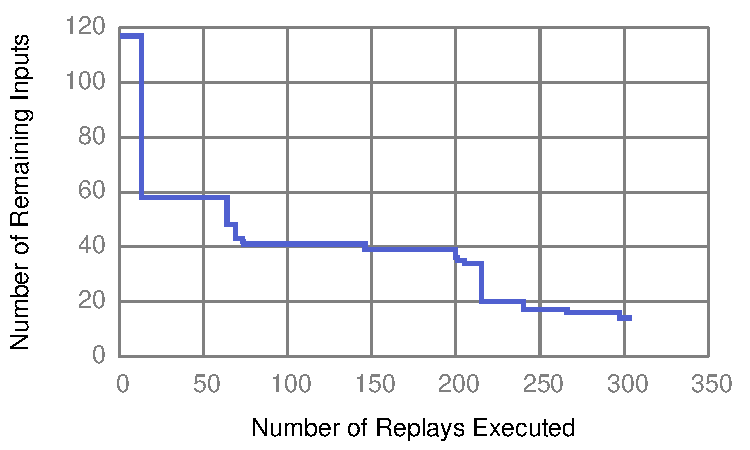
\includegraphics[width=3.25in]{../graphs/runtime/floodlight_loop.pdf}
    \caption[]{\label{fig:fl_loop} Minimizing the Floodlight loop.}
\end{figure}

We repeatedly replayed the 13 event MCS, while successively adding
instrumentation and increasing the log level each run. After about 15 replay
attempts, we found that the problem was caused by interference of end-host
traffic with ongoing link discovery packets. In our experiment, Floodlight had
not discovered an inter-switch link due to dropped LLDP packets, causing an
end-host to flap between perceived attachment points.

While this behavior cannot strictly be considered a bug in Floodlight,
the case-study nevertheless highlights the benefit of
\projectname~over traditional fuzzing techniques: by leveraging repeated replays
of a significantly reduced MCS, we were able to diagnose the root cause--a
complex interaction between the LinkDiscovery, Forwarding, and DeviceManager
modules.

\eat{ % ------------------
We subjected the current (unmodified) open
source version of Floodlight (git commit f37046a) to fuzz testing with a three
node fully meshed topology and high failure event rates. In an hour-long experiment,
the fuzzer found an event sequence with $284$ total events
that results in a 3-node forwarding loop.

Floodlight makes use of multiple kernel level
threads, and thus can exhibit non-deterministic behavior.
Thus, it is not surprising that we do not achieve full reproducibility of this
bug during replay without further instrumentation. On average, 15/50 (30\%) of
replays reproduce the bug. To proceed with MCS isolation, we replayed the
execution up to 13 replays for each subsequence chosen by delta debugging. Statistically, this enables
STS to correctly diagnose violations in >99\% of cases.\footnote{$ln( 1 -
0.99) / ln( 1 - 0.30) \approx 13$}

\projectname~was able to reduce the number of input events to $36$ input events.
Comparing output traces of successful and
unsuccessful runs, we noticed that the bug seems to correlate with specific
thread level race conditions between state updates in the \emph{LinkDiscovery} module and
the \emph{Forwarding} module. We are in the process of investigating the actual root cause.

This experiment provides a baseline for a worst case scenario of our system.
\projectname~exercised an unmodified, multithreaded controller that it does
not have deterministic control over.
The bug appears to depend on fine-grained thread-level races
conditions that are difficult to guarantee. Still, \projectname was instrumental
in pointing out a previously unknown bug, and reducing the input size.
} % ----------------------

\subsection{Known \& Synthetic bugs}

In addition to our troubleshooting case studies, we evaluate
\projectname's ability to minimize traces on a range of bug types,
both known and synthetically injected by us.

\noindent{\bf Floodlight example failover bug.}  We were able to reproduce a
known problem in Floodlight's distributed controller failover logic~\cite{floodlight_bug} with
\projectname. In Floodlight switches maintain one hot connection to a master controller and
several cold connections to replica controllers. The \emph{master} holds the
authority to modify the configuration of switches, while the other
controllers are in \emph{backup} mode and do not change the
switch configurations. % unless they detect that the master has crashed.
If a link fails tries to connect shortly after the master
controller has died, all live controllers are in
the backup role and will not take responsibility for updating the switch
flow table. At some point when a backup notices the master failure and
elevates itself to the master role it will proceed to manage
the switch, but without ever clearing the routing entries for
the failed link, resulting in a persistent blackhole.

We ran two Floodlight controller
instances connected to two switches, and injected 200 extraneous link
and switch failures, with the controller crash and switch connect event\footnote{We used a switch connect
event rather than a link failure event for logistical reasons, but both
can trigger the race condition} that triggered the blackhole interleaved among them.
We were able to successfully isolate the two event MCS: the controller crash
and the link failure.
%On ten repeated runs, the algorithm successfully pruned all extraneous
%inputs despite non-determinism in the Floodlight internal events. With full determinism and
%interposition, we expect that the algorithm should work well for less
%fabricated cases.

\eat{
We introduce our approach using an example bug in the Floodlight open-source control
platform~\cite{floodlight_bug}. Floodlight is distributed across
multiple controllers for high availability, and provides support for
virtualization. Switches maintain one hot connection to a master controller and
several cold connections to replica controllers. The \emph{master} holds the
authority to modify the configuration of switches, while the other
controllers are in \emph{backup} mode and do not change the
switch configurations unless they detect that the master has crashed.

\begin{figure}[t]
  %\hspace{-10pt}
  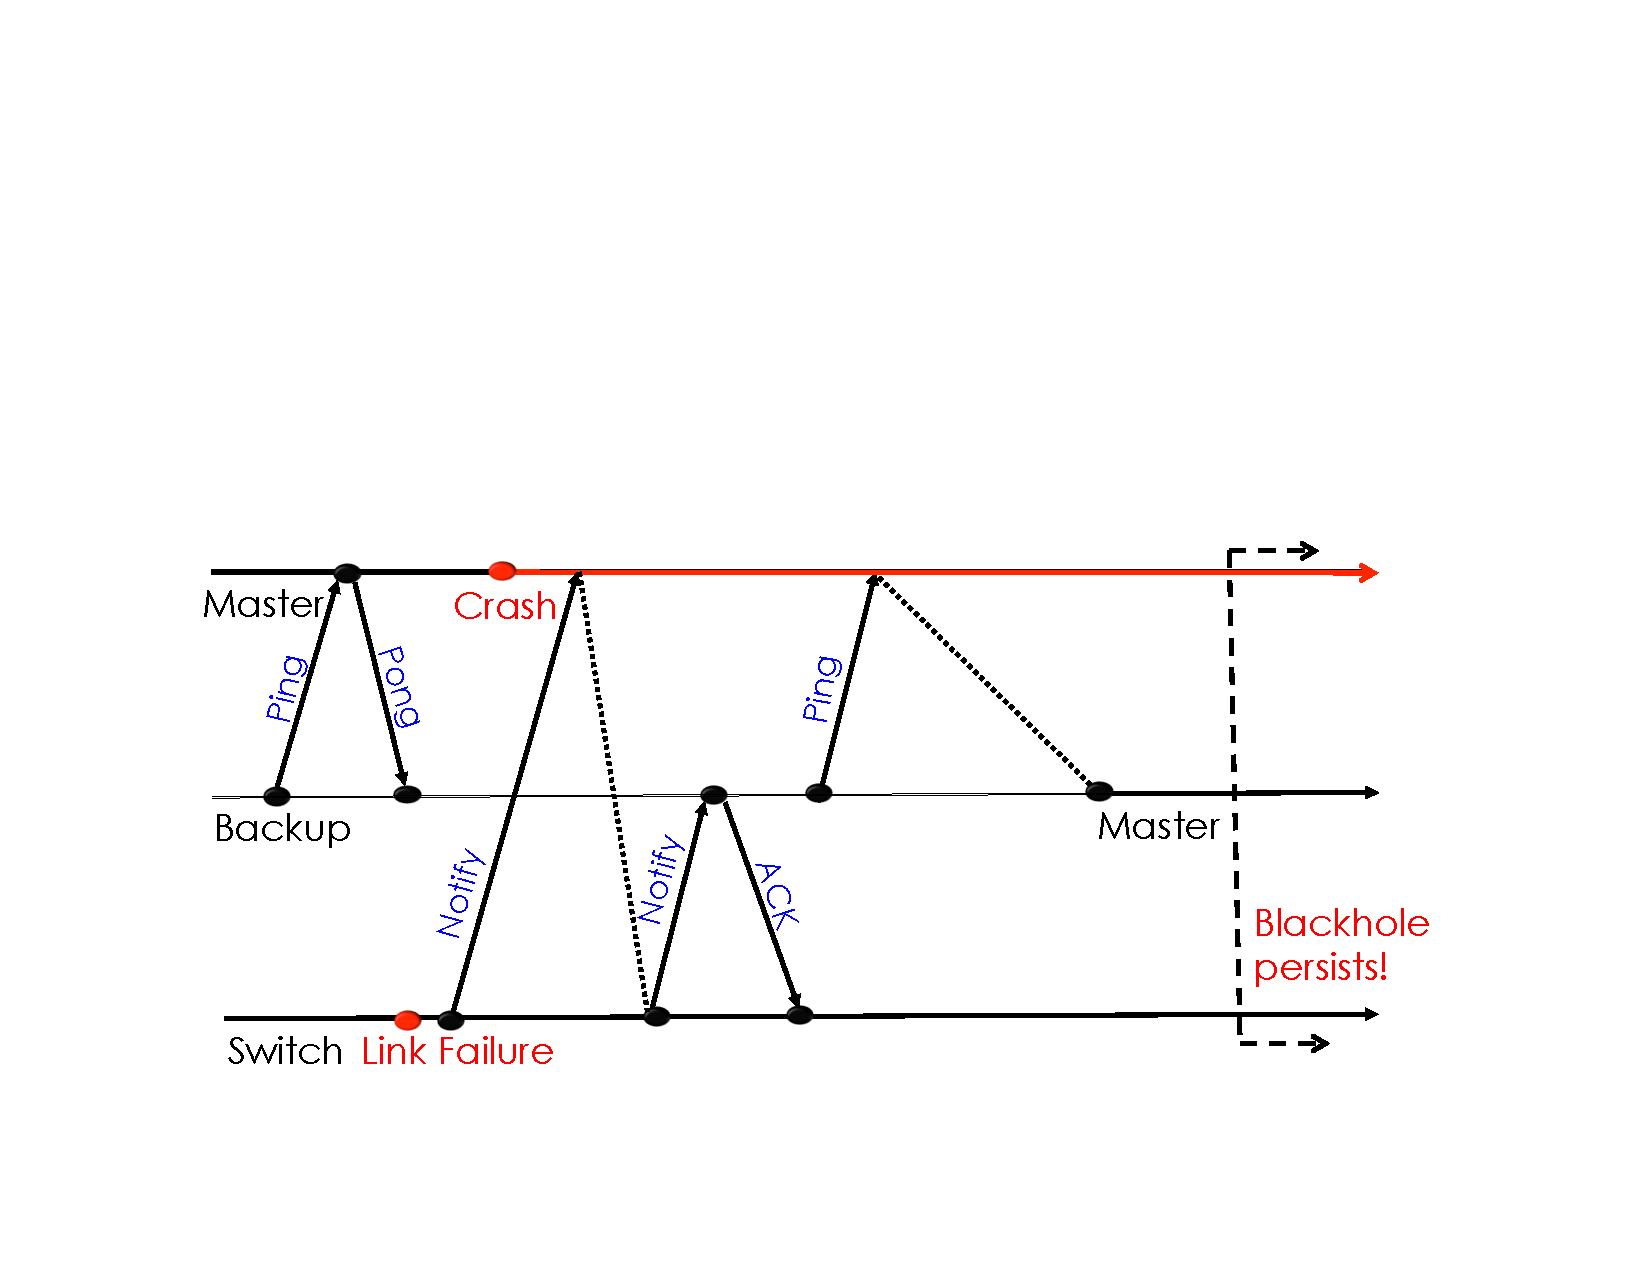
\includegraphics[width=3.25in]{../diagrams/case_study/example_bug.pdf}
  \caption[]{\label{fig:example} Floodlight failover bug. External inputs
             are depicted as red dots, internal events are depicted as black
             dots, and the dotted message line depicts a timeout.}
\end{figure}

The failover logic in Floodlight is incorrect, leading to the
following race condition\footnote{Note that this issue was
originally documented by the developers of Floodlight~\cite{floodlight_bug}.} depicted in
Figure~\ref{fig:example}:
a link fails (E1), and the switch attempts to notify the controllers (E2,E4) shortly after the master
controller has died (E3), but before a new master has been selected (E6). In this case, all live controllers are in
the backup role and will not take responsibility for updating the switch
flow table (E5). At some point, a backup notices the master failure and
elevates itself to the master role (E6). The new master will proceed to manage
the switch, but without ever clearing the routing entries for
the failed link, resulting in a persistent blackhole. In this example, the MCS
is the conjunction of the two external inputs (E1,E3).
}

\noindent{\bf ONOS master election bug.} We reproduced another bug,
previously reported in earlier versions later fixed, in
ONOS' master election protocol. If two adjacent switches are connected to two
separate controllers, the controllers must decide between themselves who will
be responsible for tracking the liveness of the link. They make this decision
by electing the controller with the lower ID as the master for that link.
When the master dies, and later reboots, it is assigned a new ID. If
its new ID is higher than the other controllers', a transient problem will
occur where both will incorrectly
believe that they are not responsible for tracking the liveness of the link,
and not routes will traverse it. We managed to reproduce this situation with
\projectname~and minimize the MCS for it: \num{TBD.}

\noindent{\bf POX Load Balancer Error Checking.} We are aware that POX
applications do not always check error messages sent by switches
rejecting invalid packet forwarding commands. We used this to trigger a bug in
POX's load balancer application: we created a network where switches had only
25 entries in their flow table, and proceeded to continue injecting TCP flows
into the network. The load balancer application proceeded to install entries
for each of these flows.At a certain point the switches ran out of flow entry
space, and responded with error messages. As a result, POX began randomly load
balancing each subsequent packet for a given flow over the servers, causing
session state to be lost. We were able to able to minimize the MCS for this
bug to 24 elements (two auxiliary flow entries, plus 22 flow needed to
overflow the routing tables). An interesting aspect of this MCS is that its
sisze is directly proportional to the flow table space, and developers would
find across across many fuzz runs triggering that the MCS was always 24
elements.

\noindent{\bf Synthetic bugs}

Lastly, we injected synthetic bugs across of bug types into POX. For space
reasons we only briefly describe these bugs.

\noindent{\bf Delicate timer interleaving}
We injected a crash into a code path that was highly dependent on the
interleaving of internal timers going off within POX. This is a particularly
hard case for \projectname, since we have little control of internal timers.
We were able to trigger the code path during fuzzing, but were unable to
reproduce the bug during replay after five attempts, and were left with the
original 39 input trace. This is the only bug we encountered that we were
unable to replay.

\noindent{\bf Algorithm misimplementation}
We modified POX's implementation of Floyd-Warshall to create loops.
We noticed that the MCS was inflated by at least two events: a link failure
and a link recovery that we did not belive were relevant to trigger the bug we
induced. Moreover, the final MCS was not replayable on the first try.
We suspect that these problems may have been introduced by the fact that the
routing implementation depended on the discovery module to find links in the
network, and the order in which these links are discovered is
non-deterministic.

\noindent{\bf Overlapping flow entries}
We ran two modules in POX: a capability manager in charge of providing
upstream DoS protection for servers, and a forwarding application. The
capabilities manager installed drop rules upstream for servers that requested
it, but these rules had lower priority than the default forwarding rules in
the switch. We were able to minimize 27 inputs to the two traffic injection
inputs necessary to trigger the routing entry overlap.

\noindent{\bf Null pointer on rarely used codepath.}
On a rarely used-code path, we injected a null pointer exception,
and were able to successfully minimize a fuzz trace of 365 events to the
expected conditions that triggered that code path: a switch failure followed
by a switch recovery.

\noindent{\bf Multithreaded race condition}
We created a race condition between multiple threads in POX that was
triggered by any packet I/O, not any particular input. With 5 replays per
subsequence, we were able to minimize 1596 input in 10 hours 15 minutes to a
replayable 2 element failure/recovery pair as an MCS.
The MCS itself may have been misleading to a developer, as the race condition
was triggered randomly by any I/O, yet the bug was still tickled by these two
inputs events.

\noindent{\bf Memory Leak}
We created a case that would take \projectname~very long to minimize: a
memory leak that eventually caused a crash in POX. We artificially set the
memory leak to happen quickly after allocating 30 objects created upon switch
handshakes, and interpersed 691 other input events throughout switch reconnect
events. The final MCS found after 4 hours 15 minutes was exactly 30 events, but it
was not replayable. We suspect this was because \projectname~was timing out on
some expected internal events, which caused POX to reject later switch
connection attempts.

\noindent{Memory Corruption}
We simulated a case where the receipt of
link failure notification on a particular port causes corruption to an internal data
structure. This corruption then causes a crash when the data structure is
accessed during the during corresponding port up. These bugs
are often hard to debug, because considerable time can pass between the event
corrupting the data structure and the event triggering the crash, making
manual log inspection or source level debugging ineffective.
\projectname~proved effective in this case, reducing a larger trace to
exactly the 2 events responsible for the crash.

\subsection{Overall Results}

The overall results of our case studies are
shown in Table~\ref{tab:case_studies}.
\num{We show the initial input size and MCS input size in the last two
columns.}
For the Replay Success Rate column we
repeatedly replayed the original unpruned event trace, and measured how often we
were able to reproduce the policy violation. There was indeed non-determinism
in some cases, especially Floodlight. For the specific case of
POX in-flight blackhole, we were able to eliminate the relevant
non-determinism by employing multiplexed sockets, overriding {\tt
gettimeofday()}, and waiting on
POX's logging messages. \num{We expect that we would see similar improvements if we
applied these techniques to Floodlight.}

We measured the runtime of \projectname~for these case studies in Figures
\num{$6\;\&\;8-11$}.
While some instances ran in logarithmic time, the worst case was minimizing
the Floodlight loop,
which took more than $8.5$ hours.
%Nonetheless, we believe that even long minimization runtime
%is preferable to spending software developer's time on manual
%diagnosis.

%\subsection{Mitigating Non-Determinism}
%
%Our implementation of multiplexed sockets and
%Include how many lines it took to interpose on the logging library, and how
%many lines it took to answer snapshot requests.

%\subsection{Peek effectiveness}
% How well does peek() work vs. only the heuristics?

%\subsection{Replaying multiple times to mitigate non-determinsm}
% How well does it work? -> Andrew

%\subsection{New Internal Events}
%
%How often do unexpected internal events occur in practice?
% The logging statements must also contain enough context[d] to allow for
% unambiguous fingerprinting. -> what exactly this means

\subsection{Instrumentation Complexity}

For POX and Floodlight, we added shim layers to the controller software to
to redirect {\tt gettimeofday()} to \projectname~and interpose on logging
statements. For Floodlight we needed 722 lines of Java to obtain this
indirection, and for POX we needed 415 line of Python.

%andi@aquil-vm:~/entw/openflow/floodlight-sts$ git diff --stat f37046a..HEAD | grep '|' | grep -v 'slf4j' | grep .java | grep sts | perl -pai -e '$sum += $F[2]; END { print $sum, "\n"; }'
% .../aspects/sts/HorribleMicroSecondTimeSource.java |   92 +++
% src/main/aspects/sts/MicroSecondTime.java          |   54 ++
% src/main/aspects/sts/MicrosecondTimeSource.java    |    7 +
% src/main/aspects/sts/SimpleLogger.java             |   44 ++
% src/main/aspects/sts/SyncMessageDecoder.java       |   34 +
% src/main/aspects/sts/SyncMessageEncoder.java       |   29 +
% src/main/aspects/sts/sync/StsSyncModule.java       |   53 ++
% src/main/aspects/sts/sync/StsSyncService.java      |  192 +++++
% src/main/aspects/sts/sync/message/StateChange.java |   42 ++
% src/main/aspects/sts/sync/message/SyncMessage.java |   59 ++
% .../sts/sync/message/SyncMessageBuilder.java       |   75 ++
% .../sts/HorribleMicroSecondTimeSourceTest.java     |   41 ++
%722

%cs@yossarian:~/Research/UCB/code/sts/sts/syncproto$ wc -l *py
%      15 __init__.py
%     215 base.py
%     205 pox_syncer.py
%     430 total

\subsection{Coping with Non-determinism}

The most elusive class of bugs comprises of those that are not always reproducible. These bugs are
usually highly dependent on the specific timings of the sequence of relevant events, either
across threads or across nodes. This limits the effectiveness of \projectname{} to minimize the
size of the MCS, as the underlying algorithm relies on the ability to successfully replay
invariant violations.

To mitigate the effects of non-determinism, we replay the given sequence of events multiple times
during MCS computation. This approach is motivated by the following observation: the probability
of failure in reproducing an invariant violation diminishes at a rate of $(1 - x)^n$, where $x$ is
the probability of success, and $n$ the number of replays. As an example, after 10 replays, a
sequence that triggers a violation with a probability of $0.5$ now has a probability of less than
$0.001$ of failure in reproducing the violation.

We evaluate the effectiveness of this approach on the MCS computation of a non-deterministic Floodlight
loop. Figure~\ref{fig:non-determinism} demonstrates that the size of the resulting MCS decreases
exponentially with the number of replays. This is because the algorithm narrows its search every time
the expected violation is triggered; replaying a subsequence multiple times significantly improves its
likelihood of successfully reproducing the violation.

\begin{figure}[t]
    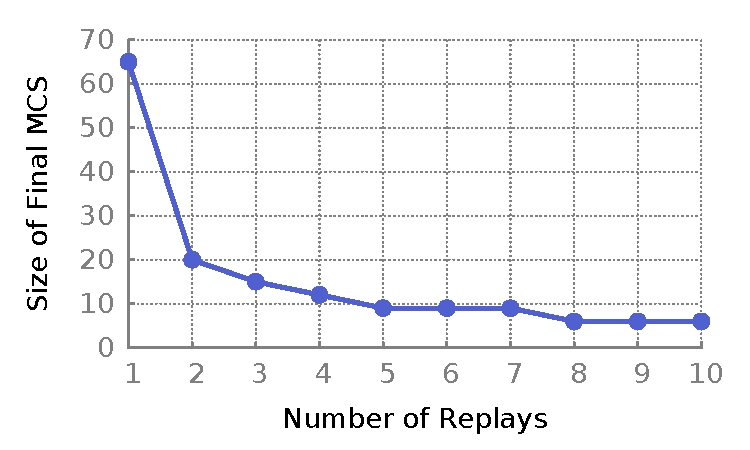
\includegraphics[trim=0 0.5cm 0 0, width=3.25in]{../graphs/non-determinism/replays.pdf}
    \caption[]{\label{fig:non-determinism} Effect of replaying a sequence multiple times on
non-determinism during MCS computation.}
\end{figure}

\subsection{Scalability}

Mocking the network in a single process potentially prevents \projectname~from
triggering bugs that only appear at large scale. We ran
\projectname~on large FatTree networks to see where these scaling limits lie.
On a machine with 6GB of memory, we ran POX as the controller, and measured the
time to create successively larger FatTree
topologies, complete the OpenFlow handshakes for each switch,
cut $5\%$ of links, and process POX's response to the link failures. As shown in
Figure~\ref{fig:scaling}, \projectname's processing time scales roughly
linearly up to $2464$ switches (a 45-pod FatTree). At that point, the machine
started thrashing, but this limitation could easily be removed by running on a
machine with >6GB of memory.

Note that \projectname~is not designed for simulating high-throughput dataplane
traffic; we only forward what is necessary to exercise the controller
software. In proactive SDN setups, dataplane events are not
relevant for the control software, except perhaps for host discovery.

\begin{figure}[t]
    %\hspace{-10pt}
    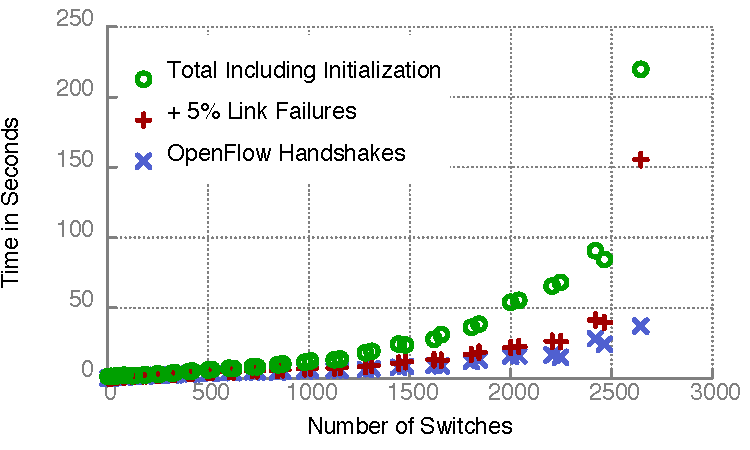
\includegraphics[width=3.25in]{../graphs/scalability/scaling.pdf}
    \caption[]{\label{fig:scaling} Simulation time for bootstrapping FatTree
    networks, cutting 5\% of links, and processing the controller's response.}
\end{figure}

\subsection{Parameters}
\label{subsec:params}

We found throughout our experimentation that \projectname~leaves open several
parameters that need to be set properly in order to effectively find and troubleshoot bugs.

\noindent{\bf Setting fuzzing parameters.} \projectname's fuzzer allows the
user to set the rates at which different event types are triggered. In our experiments with
\projectname~we found several times that we needed to set these parameters
such that we avoided bugs that were not of interest to developers.
For example, in one case we discovered that a high dataplane
packet drop rate dropped too many LLDP packets, preventing the controller from ever successfully discovering the topology.
Tweaking fuzzing parameters remains an important
part of experiment setup.

\noindent{\bf Differentiating persistent and transient violations.} In
networks there is a fundamental delay between the initial occurrence of an
event and the time when other nodes are notified of the event. This delay implies
that invariant violations such as loops or blackholes can appear
before the controller(s) have time to correct the network configuration. In
many cases such transient invariant violations are not of interest to
developers. We therefore provide a threshold parameter in \projectname~for
how long a invariant violation should persist before
\projectname~reports it as a problem. In general, setting this
threshold will depend on the parameters of the network and the invariants of
interest.

\noindent{\bf Setting \textepsilon.} Our algorithm leaves an open question as to what value
\textepsilon~should be set to. We experimentally varied \textepsilon~on the
POX in-flight blackhole and the POX list removal bugs.
We found for both cases that the number of events we timed out on while isolating the MCS became stable for values above $25$ milliseconds.
For smaller values, the number of timed out events increased rapidly. We
currently set \textepsilon~to $100$ milliseconds.

In general, larger values of \textepsilon~are preferable to
smaller values (disregarding runtime considerations), since we can always
detect when we have waited too long (\viz~when a successor of the next input
has occurred), but we cannot detect when we have timed out
early on an internal event that is in fact going to occur shortly after.

%\colin{Make me work}
%\begin{table*}
%\centering
%\begin{tabular}{l|l|l|l|l|l}
%Bug Name & \textepsilon & \textepsilon & \textepsilon & \textpsilon &
%\textepsilon \\
%\hline
%POX list removal (Replay) & 59.3\% & 98.0\% & 98.3\% & 98.3\% & 98.5\% \\
%POX list removal (MCS) & 58.3\% & 69.9\% & 69.9\% & 70.6\% & 70.9\% \\
%POX in-flight blackhole (Replay) & 24.4\% & 100.0\% & 100.0\% & 100.0\% & 100.0\% \\
%POX in-flight blackhole (MCS) & 24.0\% & 75.9\% & 75.9\% & 75.9\% & 75.2\% \\
%\end{tabular}
%\caption{Percentage of Events Matched for Values of \textepsilon in ms.}
%\label{tab:epsilon}
%\end{table*}

%Analyzing event frequencies for particular bugs could provide more ideal
%\textepsilon~values.

% ------------------------------------- %
%    OLD TEXT
\eat{ % -----------------------------------

% Just realized: b/c of anonymity, the PC can't chastise us for
% running our system on our own code -- we can't tell them that it's our code!
We applied \projectname{} to three open source SDN control platforms:
Frenetic~\cite{frenetic}, POX~\cite{pox}, and Floodlight~\cite{bigswitch}, and
quickly found (or reproduced) one bug in each. The bug in Frenetic demonstrates
the utility of checking correspondence between high-level policies and
low-level configuration (without needing to specify invariants). The bugs in
POX and Floodlight demonstrate the importance of \projectname{}'s ability to
programmatically prioritize persistent correctness violations and infer their minimal
causal sets.

For all three cases, only a small code modification to the controller was necessary
to retrieve the platform's state for correspondence
checking.

\subsection{Case studies}

% Outline for bug reports:
%  - Describe each system under test
%  - Describe bugs found
%  - Lessons learned from finding bugs
Here we the discuss the three bugs we found with \projectname{}.

\noindent{\bf Frenetic.} Our first example is Frenetic~\cite{frenetic}, a control platform
providing functional-reactive language
support for programming OpenFlow networks.
Frenetic's language features aim to prevent common OpenFlow programming
errors such as race conditions and overlapping flow entries; Frenetic's
runtime system handles these low-level details on
the application's behalf. Frenetic is a modern SDN controller with a reactive
flow installation policy;
we present it here to demonstrate that \projectname{}, although focused
primarily on proactive controllers, can nonetheless be used to
troubleshoot errors in reactive control platforms.

When running learning switch, the simplest Frenetic application, we encountered
persistent correctness violations immediately. The propagation graph ($\Omega$) for Frenetic's
runtime representation of the network policy had leaves that were not present
in the physical network. Upon closer examination, we found that Frenetic's
runtime system was neglecting to remove old FLOOD routing entries from its
representation of the network policy after the hosts' route had been learned,
even though the learning switch application had
asked for these entries to be removed. Note that this case was not an overtly
malicious bug; the FLOOD entries had indeed been removed from the physical
network. The outdated controller state nevertheless went unnoticed; the bug in
Frenetic's runtime was not specific to the learning switch, and could have
resulted in failure to install flow entries at a later point in time if the
application had asked to re-install them. The key takeaway from this example
is that correspondence checking is a powerful mechanism for
verifying that the controller's representation of the network matches the true
network state correctly; without correspondence checking, troubleshooters
would need to compare the routing configurations and controller's data
structures side-by-side.

\noindent{\bf POX} Our second example is POX~\cite{pox}. POX is modeled after
Onix~\cite{onix}, a production SDN platform; as in Figure~\ref{fig:basicarch}
POX provides a physical view, a virtualized view, and a naive replication
mechanism between distributed control servers.

Because the functionality within POX is relatively young, we chose to
fabricate a bug in POX's distribution failover logic, and independently
validate that \projectname~was able to identify, prioritize, and find the
minimal causal sequence for the fabricated correctness violation.

In particular, we injected the following bug: a controller replica performs
updates to switches by (i) updating the persistent datastore storing the state
of the network (thereby notifying other replicas of the update), and (ii) pushing the
update to the switch. A control server writes a new ACL entry update to the datastore, but crashes
before completing step (ii). The switch is adopted by a new replica,
but the new control server assumes that the state in the persistent datastore
is correct. The ACL entry is therefore never installed in the switch, and a
breach of tenant isolation occurs.

We interleaved this event sequence with a normal system execution trace, and
determined whether \projectname{} could identify the correctness violation.
Throughout the system execution there were a handful of transient
correctness violations overlapping with the isolation breach. Nonetheless, our
simulator was able to identify the correct correctness violation.

\noindent{\bf Floodlight: Distributed controller failover race condition}
We were able to reproduce the problem shown in Figure~\ref{fig:example} in our
simulation environment,\footnote{The code is publicly available}
and apply \projectname~successfully.
We modified the Floodlight software to provide an interface for extracting its
physical view. We did not interpose on internal events of the controller, but instead used a
heuristic to wait for $.5$ seconds between injecting inputs to allow the
controllers to fully react. We ran two of the modified Floodlight controller
instances, connected to two simulated switches, and injected 200 extraneous link
and switch failures, with the controller crash and switch connect event\footnote{We used a switch connect
event rather than a link failure event for logistical reasons, but both
can trigger the race condition} that triggered the blackhole interleaved among them.
On ten repeated runs, the algorithm successfully pruned all extraneous
inputs despite non-determinism in the Floodlight internal events. With full determinism and
interposition, we expect that the algorithm should work well for less
fabricated cases.

\subsection{Overhead}

\colin{Reviewer OB: I would prefer to see a more in-depth analysis of why
correspondence checking is not as heavyweight as, say, conventional
model-checking. Is it the inherent symmetry in data center networks? Can we
assume that there is symmetry?}

In addition to describing bugs, we show that \projectname{} is able
to simulate and check large networks quickly.

\noindent{\bf Record and Replay Overhead.} In contrast to general record-and-replay
mechanisms, the amount of recorded state needed for
high-fidelity replay is tractable. With proactive flow installation,
updates are pushed to routing tables over a relatively long time scale; periodic
FIB snapshots along with a log of link state events, control server
downtime, and host mobility information suffice for our purposes. As a point of reference, the Cisco 7000
core switch model supports a maximum of 128K MAC entries and
128K ACL entries~\cite{cisco7000}. Assuming 36 bytes per flow entry,
(larger than the OpenFlow 13-tuple), each FIB will contain a maximum of 9216
bytes, uncompressed. A datacenter of 100,000
hosts includes roughly 8,000
switches~\cite{Al-Fares:2008:SCD:1402958.1402967}.
Therefore a snapshot of the FIBs of the entire network takes up roughly 74 MB.
The VL2 paper reports 36M network error events over one year over 8
datacenters, which implies 8.5 error events per minute per
datacenter~\cite{Greenberg:2009:VSF:1592568.1592576}.
Suppose we took a snapshot of the FIBs in the network every second.
Then we would need to store roughly 4GB, uncompressed, per minute, a relatively small growth
rate for datacenter logs. This information, in addition to a log of host
mobility events (\eg{} VM migrations) will suffice for our purposes. Note that this is a conservative overestimate.

\colin{Notes from Rean Griffith:
\begin{itemize}
\item total vms in a typical datacenter: 1000
\item migration frequency (migrations/minute): 20 per hour
\item VM spin ups/downs: 150 power ons per hour (see our OSR 2010 paper for
power off estimates)
\item Do we log VM migrations and how does that log grow (I wasn't able to
get any estimates on log-growth data)
\end{itemize}

We had an OSR 2010 paper that provided numbers scaled by the number of
VMs in an installation:
Challenges in building scalable virtualized datacenter management
(http://dl.acm.org/citation.cfm?id=1899941)
}

%To account for host mobility, assume that each server hosts 10 VMs,
%and 1\% of VMs are created, suspended, or migrated every minute. Then 10,000 host mobility events must be
%logged per minute, also a reasonable storage cost. \colin{get real numbers}

%As a point of reference, border routers' working RIB size is
%$\textasciitilde$130MB~\cite{Karpilovsky:2006:UFR:1368436.1368439}.

\noindent{\bf Correspondence Checking Runtime.} Computing the propagation
graph for correspondence checking is equivalent to enumerating
all possible paths in the network, which scales with the diameter
of the network and the number of routing entries per switch \colin{Reviewer
OC: scales how? I suspect it's at least N2}.
The propagation graph for each host can be
computed in parallel however, so the computation is bottlenecked by the serial runtime
of computing a single host's propagation graph.

We show the serial runtime of correspondence checking in
Figure~\ref{fig:hsa_runtime}. For this analysis we generated fat tree topologies
between 2 and 48 pods wide, with pre-installed PORTLAND~\cite{NiranjanMysore:2009:PSF:1592568.1592575}
routing tables in each switch. Each data point is the minimum of three
runs\colin{Reviewer OC: seems to overstate value of approach if maximum is much different} on a single Intel Xeon 2.80GHz core. Note that the number of PORTLAND routing entries per switch scales with the number
of pods in the fat-tree. We excluded the time to convert
flow tables to HSA transfer functions, since transfer functions can be maintained
offline.

\colin{Reviewer OB:  what are the characteristics of the PORTLAND routing
table? If the tables were any different, would the performance of
correspondence checking remain the same, degrade or improve? }

\colin{Reviewer OD: First the paper started generally, then it narrows its
scope to PORTLAND-style datacenters. An accurate abstract would have reflected
this narrowing of scope}

As the figure depicts, even for large networks
(27,648 hosts) the serial runtime of correspondence checking is reasonable for
interactive use. The number of serial tasks to be executed
is the number of hosts in the network squared, disregarding ECMP load balancing.
\colin{reviewer B: correspondence is not being checked. I should be clear
that this is the runtime of generating the propagation on the physical
network, which is an upper bound on the runtime of checking the virtual
network.}

\begin{figure}[t]
    %\hspace{-10pt}
    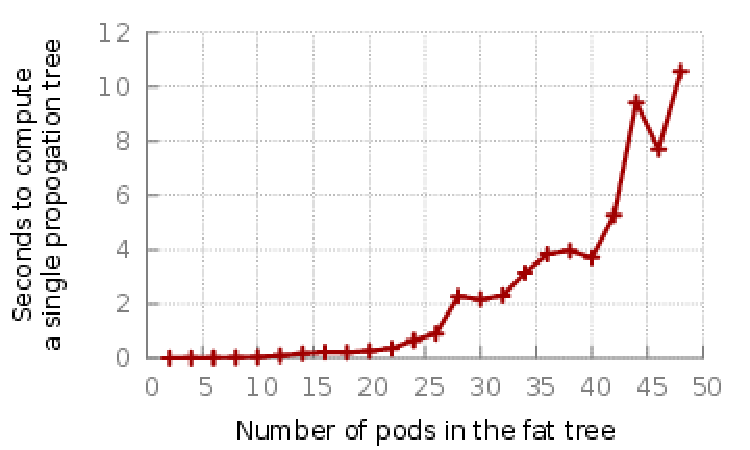
\includegraphics[width=3.25in]{../graphs/hsa_overhead_graph/graph.pdf}
    \caption[]{\label{fig:hsa_runtime} Serial runtime of correspondence
    checking on PORTLAND fat tree networks. Each datapoint consists of
    $x^3/4$ hosts and $5x^2/4$ switches (\eg{} 48 pods means 27,468 hosts
    attached to 2,880 switches)}
\end{figure}

\noindent{\bf Simulator Scalability.} Our design models the entire network
within a single process. We show in Figure~\ref{fig:scalability}
that this approach nonetheless scales to large networks. For this analysis we
generated fat tree topologies between 2 and 48 pods wide, where all switches in
the network connected to a single controller. The controller sent each switch
an OpenFlow
$FLOW\_MOD$ and subsequent $BARRIER\_REQUEST$ message, and waited for the
corresponding $BARRIER\_REPLY$. We then measured the time to between the first
$FLOW\_MOD$ sent and the last $BARRIER\_REPLY$ received. As expected, the
runtime was roughly linear with the number of switches in the network. The
figure also shows that the processing time for large networks (5 seconds per
simulator round) was well within the bounds for interactive use.

\begin{figure}[t]
    %\hspace{-10pt}
    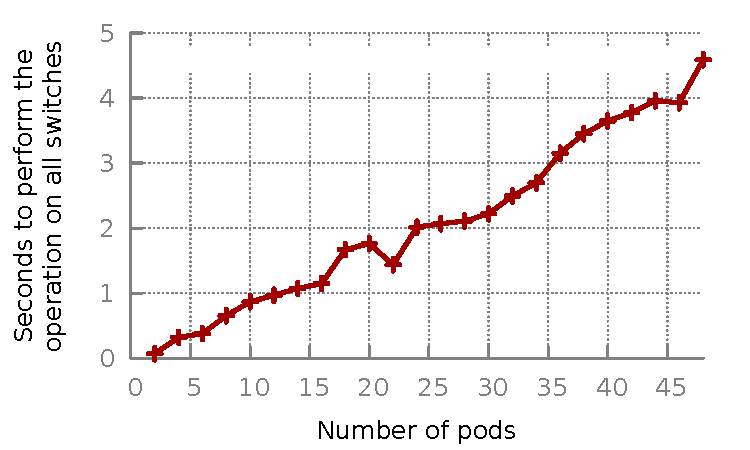
\includegraphics[width=3.25in]{../graphs/scalability_graph/scale.pdf}
    \caption[]{\label{fig:scalability} Time to send and process messages
    between controller and simulated switches. Each datapoint consists of
    $x^3/4$ hosts and $5x^2/4$ switches (\eg{} 48 pods means 27,468 hosts
    attached to 2,880 switches)}
\end{figure}

We also tested the extreme limits of the simulator's scalability, pushing up
the number of switches until something broke. We encountered what appears to be
a limitation of the Linux TCP/IP stack: TCP connection attempts began failing
beyond 26,680 sockets. Note that 26,680 switches is an order-of-magnitude larger than
the today's biggest networks.

\subsection{Replay fidelity}

On the one hand, since the SDN platform is in software, we can, in theory,
reproduce all software-induced policy violations (though not problems
resulting from flaky hardware implementing code incorrectly). However, this
requires setting up the simulator to emulate the appropriate conditions that
led to the policy violation, and that can be quite difficult. We hope to make
progress in this area along two dimensions.  First, we hope to help the
community build up a set of regression tests, so that a wide variety of
bug-triggering scenarios are available in a public repository. This would go a
long way towards providing adequate test coverage.

Second, we hope to gather error logs from real production deployments which
will help us populate this repository; this may require providing novel kinds
of anonymization, so that large datacenter operators would be willing to share
their problems (since they want their SDN code to work) without revealing the
details of their network.  This may require a infrastructural counterpart to
minimally-causal events; the smallest number of infrastructure components that
can reproduce the same bug.

Also, note that our correspondence checking algorithm can not verify
time-dependent policies such as ``No link should be congested more than 1\% of
the
time'', or ``No server should receive more than 500MB/s of external traffic''.
In future work we will extend our correspondence checking algorithm to
account for this class of policies.

\colin{reviewer B: in fact, in addition to temporal properties, the
correspondence checking algorithm cannot verify any properties involving
individual links since it only accounts for externally observable behavior!}
}    % -----------------------------------
